\chapter{Methods}
\label{ch:methods}

\section{Overview}
\label{sec:overview}
Our objective is to evaluate the capacity of existing LiDAR place recognition models to successfully provide robust loop closure candidates within dense forest environments. Our evaluation considers three distinct tasks: 
\begin{itemize}
  \listparindent=-20pt
  % \itemindent=-10pt
  \item \emph{Task A: Online SLAM}: the proposed loop candidates contributing to a globally-consistent pose graph mapping system in an incremental manner.
  \item \emph{Task B: Offline multi-mission SLAM}: loop candidates used to link different physically overlapping missions collected at different times.
  \item \emph{Task C: Relocalization}: place recognition in a prior map made up of individual scans enabling autonomy within the map such as longer term monitoring or harvesting.
\end{itemize}

Our system infrastructure is shown in \figref{fig:pipeline}. For state estimation, we use a LiDAR-inertial odometry system---VILENS~\cite{wisth2023tro}---, in conjunction with a pose graph SLAM framework~\cite{proudman2022ras}. Additionally, we implemented a \emph{place recognition \& verification server}, which not only provides a common interface for the different LiDAR-based place recognition models but also multi-stage verification procedures for its use in the different proposed tasks.
In the following sections, we present the technical details of the place recognition server, and then we present its integration to solve the three aforementioned tasks. 


\begin{figure}[t]
  \centering
  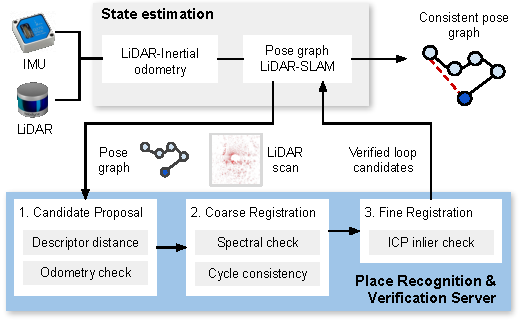
\includegraphics[width=\columnwidth]{pics/method_pipeline.pdf}
  \caption{Our place recognition pipeline. VILENS provides a continuous odometry estimate at 10 Hz. Pose graph SLAM is used to optimize poses after successful loop closure verification. 
  The place recognition module consists of three steps: Loop candidate proposal, coarse registration, and fine registration. We verify loop candidates
  at the global descriptor-level, local feature-level consistency, and finally fine registration level. A loop candidate is integrated in the pose graph only if it passes these three stages.}
  \label{fig:pipeline}
\end{figure}

\section{State Estimation}
State estimation module provides the robot's pose estimate at each time step based on sensor measurements. We use a LiDAR-intertial odometry system called VILENS~\cite{wisth2023tro} to provide a continuous odometry estimate at high frequency. The odometry system is used to provide a prior estimate of the robot's pose, which is then optimized globally using a pose graph SLAM system. We will provide a brief overview of the odometry system and the pose graph SLAM system in the following paragraphs. 

\subsubsection*{\textbf{LiDAR-intertial Odometry}} 
For our odometry system, we use a LiDAR-intertial factor graph-based odometry system, VILENS~\cite{wisth2023tro}. \figref{fig:vilens_factorgraph} left image shows odometry of VILENS as a factor graph. Particularly, VILENS provides a continuous odometry estimate at high frequency and pose displacements are computed from LiDAR using Iterative Closest Point (ICP) algorithm with preintegrated IMU information. We disabled the visual odometry factor and only used LiDAR odometry and IMU factors when running inside forest environments. 
The odometry system is used to provide a locally consistent estimate of the robot's pose. However, the odometry system can accumulate drift over long traverses. This drift should be minimized with the pose graph SLAM system by inserting loop closure constraints and optimizing the poses globally.  
\begin{figure}[t]
  \centering
  \includegraphics[width=\columnwidth]{pics/methods_vilens_factorgraph2.pdf}
  \caption{VILENS odometry system(Left) as a factor graph representation. The factors are: prior (black), visual
 (yellow), lidar planes (green), lidar lines (red), preintegrated IMU (orange), preintegrated velocity (from leg kinematics, blue), and lidar odometry (from ICP registration, magenta). State nodes are white, while landmarks are grey. In forest environments, only LiDAR odometry and IMU factors are used without visual factors. Pose graph SLAM (Right) optimizes the poses after successful loop closure verification. The pose graph is constructed from odometry factors and loop closure factors.}
  \label{fig:vilens_factorgraph}
\end{figure}

\subsubsection*{\textbf{Pose graph LiDAR SLAM}}  We use a pose graph SLAM system to optimize the robot's pose estimate. The pose graph is constructed from odometry factors and loop closure factors as shown in \figref{fig:factor_graph}. Each node contains a LiDAR scan and corresponding pose, and the edge is formed between consecutive nodes from incremental odometry estimates. Additionally, loop closure adds another constraint between two nodes. The odometry factors are provided by VILENS, while the loop closure factors are obtained from the place recognition server. The pose graph is optimized using iSAM2~\cite{Kaess2012} algorithm. 

The pose graph is used to provide a globally consistent pose estimate by jointly optimizing all poses in the graph when there is a loop closure. For example, \figref{fig:odometry_slam} shows illustrative examples of the odometry path (yellow line) and optimized SLAM path (green line) after long traverses in forest environments and came back to the starting point. Loop closure (red line) at the end of the traverse is used to correct the drift accumulated in the odometry. It is clearly seen that odometry path diverges from the starting point while the optimized SLAM path is corrected this error and well aligned.

In summary, it is important to minimize accumulated drifts in the odometry system and creating globally consistent map by finding a suitable loop closure constraint. However, one incorrect loop closure can lead to a failure in the entire SLAM system. Therefore, we need a robust place recognition system to provide reliable loop closure candidates. \emph{The place recognition server} is used to provide loop closure candidates, which are then verified and integrated into the pose graph SLAM system.

\begin{figure}[htbp]
  \centering
  \includegraphics[width=0.9\columnwidth]{pics/methods_odometry_slam.pdf}
  \caption{Illustrative visualization of both odometry and SLAM paths after long traverses in Wytham Woods. The odometry path is shown in yellow line and the optimized SLAM path is shown in green. The SLAM path successfully minimized the drifts by optimizing pose graph after finding a loop closure (red line) when it came back to the starting point.}
  \label{fig:odometry_slam}
\end{figure}

% Overall Pipeline
% This star removes this subsection from the A,B,C list. Such that the task A,B,C match
\section{Place Recognition \& Verification Server} \label{sec:pipeline}
Our place recognition pipeline (\figref{fig:pipeline}) consists of three steps: loop candidate proposals, coarse registration, and a final fine-registration. At each step, we perform appropriate checks to filter out incorrect loop closures.

The main inputs are the pose graph, with corresponding LiDAR scans attached to each pose, as well as the single query scan. The query scan is provided by different sources depending on the task we are solving. For example, in the relocalization task it will be a live scan directly from the LiDAR sensor. Further details are provided in the corresponding sections.

% 1.1 Descriptors (Descriptor distance,)
\subsection*{\textbf{Step 1: Loop candidate proposals}}
\label{subsubsec:loop-candidate}
\begin{figure}[htbp]
  \centering
  \includegraphics[width=\columnwidth]{pics/methods_fig_descriptor1.pdf}
  \caption{Different types of place recognition descriptors on Wild-Place~\cite{knights2023icra} data. ScanContext(Left), STD(Middle), EgoNN and Logg3dNet(Right). ScanContext encodes maximum height at each sector(radius,angle) and compute a 2D descriptor. STD computes corners of planes (trunk of trees) and connect them to multiple triangles. EgoNN and Logg3dNet both compute learning-based pointwise descriptors in voxelized point clouds.  }
  \label{fig:descriptors_example}
\end{figure}
Initial loop closure candidates are obtained by comparing global descriptors extracted from the pose graph scans as well as the query scan. In this thesis, we evaluate four state-of-the-art methods for descriptor extraction: the learning-based Logg3dNet~\cite{vidanapathirana2022icra} and EgoNN~\cite{komorowski2022ral}, as well as the handcrafted ScanContext~\cite{kim2018iros} and STD~\cite{yuan2023icra}. \figref{fig:descriptors_example} shows their descriptors examples computed on Wild-Place data.  

Given the reference pose graph and the query scan, we compute a database of descriptors using all the scans in the pose graph, given by the matrix $\mathbf{D} \in \R{N\times M}$, where $N$ is the number of poses in the pose graph and $M$ the descriptor dimension. Additionally, we compute the descriptor for the query scan, denoted by $\mathbf{d}_{q} \in \R{M \times 1}$. 

To obtain candidates, we compute the pairwise descriptor distances of the scan to the database using the cosine similarity:
\begin{equation}
  \mathbf{S} = \mathbf{D} \cdot \mathbf{d}_{q} \in \R{N \times 1}
\end{equation}
The vector of descriptor distances $\mathbf{S}$ is sorted by increasing distance, and only the top-$k$ candidates are selecting using a distance threshold $\tau_{s}$, which is set by the $F_1$-max score from testing data.
If a spatial prior is available, for example from LiDAR-inertial odometry, we also perform an additional spatial check discarding all the candidates that are more than conservative estimate of \SI{20}{\meter} away from the query scan. The output is a set of candidate nodes $\{ n_c\}$ (We assumed that marginal covariance of the odometry is much less than \SI{20}{\meter}).


% 2.1 Pose Estimation (RANSAC) ... notation is a bit confusing.
\subsection*{\textbf{Step 2: Coarse Registration}}
\label{subsubsec:coarse-registration}
\begin{figure}[htbp]
  \centering
  \includegraphics*[width=\columnwidth]{pics/methods_registration_1.pdf}
  \caption{Registration example of two point clouds \SI{7.3}{\meter} and \SI{111}{\degree} apart. Left image is before registration. Right image shows after RANSAC-registration. After RANSAC-registration, the trunks of trees scans (Blue boxes) are clearly matched with each other . }
  \label{fig:registration_example}
\end{figure}
Next, we estimate the relative 6DoF transformation that expresses the pose associated to the query scan w.r.t each candidate node, which we denote $\Delta \mathbf{T}$. For the handcrafted methods (ScanContext and STD), the relative transformation is directly an output of descriptor computation. For the learning-based approaches, we use the point-wise feature vectors outputted in the forward pass of Logg3dNet and EgoNN for feature matching, which is used in a RANSAC-based pose estimation scheme~\cite{fischler1981ransac} to estimate the relative transformation. We used \emph{Open3D}'s RANSAC implementation~\cite{zhou2018}.  

\subsubsection*{\textbf{RANSAC Registration}}  
\figref{fig:RANSAC_keypoint_matching} shows illustrative examples of RANSAC feature matchings. We noticed that as the distance between two point clouds increases, there are more incorrect matches(outliers) due to smaller overlap between them. This also suggests that RANSAC only measures if two point clouds can be registered or not, unable to determine if a loop candidate is actually a false positive or a correct loop candidate but with far baseline distance. Therefore, we introduced two more verification layers, Spectral Geometric Verification (SGV) and pairwise cycle consistency check. 
\begin{figure}[htbp]
  \centering
  \includegraphics*[width=\columnwidth]{pics/methods_keypoint_matching.pdf}
  \caption{RANSAC matches obtained from Logg3dNet features for small and large baseline distance. Left image shows short baseline distance \SI{0.8}{\meter} and \SI{6}{\degree} viewpoint difference and right image shows large baseline distance \SI{7}{\meter} and \SI{1}{\degree} viewpoint difference. 
  The red points represent keypoints in the query point cloud, while green points depict candidate keypoints in the retrieved point cloud. Each keypoint possesses its unique feature vector, matched against the most similar feature in the retrieved point clouds (indicated by black lines). In the left image, with a short baseline distance and minimal viewpoint difference, RANSAC matching consistently discovers matching pairs along the horizontal axis. However, in the right image, where the baseline distance is significantly longer, erroneous matches become more prevalent, depicted as vertical lines.}
  \label{fig:RANSAC_keypoint_matching}
\end{figure}

\subsubsection*{\textbf{Spectral Geometric Verification (SGV)}}
We additionally verify the inlier matches using the \emph{Spectral Geometric Verification}(SGV)~\cite{vidanapathirana2023ral} method, which provides an additional measure of the quality of the feature matches. Essentially, SGV checks pairwise cycle consistency of local feature correspondences between two point clouds. Given the correspondences between two point clouds, $\mathcal{C}=\{c_1, c_2 \ldots c_n\}$ we can construct a graph $M \in \R{n \times n}$ where $M_{i,j}$ represents similarity score $s$ between $c_i$ and $c_j$. If both $c_i$ and $c_j$ are correct inliers they should be pairwise consistent in their coordinate frames with high similarity score $s$, but if one of correspondences is an outlier they will not be consistent with low similarity score $s$. 
\begin{figure}[t]
  \centering
  \includegraphics*[width=0.9\columnwidth]{pics/methods_svg_distance2.png}
  \caption{The SGV scores $s$ are computed against baseline distances and angles of loop closures obtained (White bins are empty data points). A smaller SGV score corresponds to larger baseline distances, suggesting a reduced proportion of correct correspondences. 
  For example, $s=0.1$ approximately indicates \SI{10}{\meter} baseline distance, and $s=0.05$ upto \SI{20}{\meter}. Furthermore, it was observed that the SGV score remains constant across different angles, indicating a consistent registration process irrespective of viewpoint changes (viewpoint invariant), and useful indication of baseline distance.}
  \label{fig:sgv_distance}
\end{figure}
In \figref{fig:cycle-consistency} shows the idea of pairwise cycle consistency. In this case, nodes $\{n_i, n_j, n_k, n_l\}$ represent keypoints $\{\mathbf{p_i}, \mathbf{p_j}, \mathbf{p_k}, \mathbf{p_l}\}$ where $\mathbf{p} \in \R{3}$ in own base frame, and two correspondences $c_1 =\{\mathbf{p_i}, \mathbf{p_l}\}$, $c_2=\{\mathbf{p_j}, \mathbf{p_k}\}$ are considered. Then edge between $\{n_i, n_j\}$  represents euclidean distance $\| \mathbf{p_i}-\mathbf{p_j} \|$, and similarly edge between $\{n_k, n_l\}$ will be $\| \mathbf{p_k}-\mathbf{p_l} \|$. Now we can minimise the error $d$ between these two distances to verify the quality of the feature matches considering two correspondences, $c_1$ and $c_2$. 
\begin{equation}
  d_{1,2} = |\| \mathbf{p_i}-\mathbf{p_j} \| - \| \mathbf{p_k}-\mathbf{p_l} \| | 
\end{equation}
\begin{equation}
  M_{1,2} = max( 0 , 1 - \left(\frac{d_{i,j}}{d_{\text{thres}}}\right)^2 ) 
  \quad \text{where} \quad 0 \leq M_{1,2} \leq 1 
\end{equation}
$d_{thres}$ typically set to \SI{0.1}{\meter} to \SI{0.2}{\meter} to consider the error in the registration process. If $d_{i,j}$ is larger than $d_{thres}$, we consider two correspondences are inconsistent and $M_{i,j}$ assigned to be zero.  
We then compute the total SGV score $s$ considering all correspondences $\mathcal{C}=\{c_1, c_2 \ldots c_n\}$ as follows:
\begin{equation}
  s = \sum_{i,j} M_{i,j} 
\end{equation}
By finding maximum inliers $v^{*}$, we can find the maximum SGV score $s^{*}$: 
\begin{equation}
  v^{*} = \argmax_{v} v^T M v \quad, \quad
  s^{*} = v^{*T} M v^{*}
\end{equation}
where $v$ is the eigenvector of the largest eigenvalue of $M$. The SGV score $s$ is then used to verify the quality of the feature matches.

The author of Logg3dNet proposed SGV check for reranking top-$k$ candidates obtained from descriptor distance matching in \secref{subsubsec:loop-candidate}. But, instead we used SGV for verifying registration quality against baseline distance. \figref{fig:sgv_distance} shows the SGV score computed against the distance between two point clouds. We used SGV score as an indication of baseline distance of loop candidates. For example, we set $s=0.1$ as a threshold for \SI{10}{\meter} baseline distance, and reject the loop candidates if SGV score is smaller than 0.1.



\subsubsection*{\textbf{Pairwise Loop Closures Cycle Consistency Check}}
\begin{figure}[htbp]
  \centering
  \includegraphics*[width=0.8\columnwidth]{pics/methods_pairwise_consistency.pdf}
  \caption{Our proposed pairwise cycle consistency check is general and applies to the online and offline multi-mission SLAM case, as well as relocalization tasks. We only need the relative transformation estimates and loop candidates between four nodes $n_i, n_j, n_k, n_l$ to verify the validity of a loop. Please refer to \secref{subsubsec:coarse-registration} for technical details.}
  \label{fig:cycle-consistency}
\end{figure}
Lastly, we carry out a \emph{loop closure cycle consistency} verification (\figref{fig:cycle-consistency}), which checks whether the relative transformations between pairs of nodes in pose graph are mutually consistent with one another. Given four pose graph nodes $n_i, n_j, n_k, n_l$, we test how close the following equivalence holds:
\begin{equation}
\Delta\mathbf{T}_{i,j}\, \Delta\mathbf{T}_{j,k}\, \Delta\mathbf{T}_{k,l}\, \Delta\mathbf{T}_{l,i}\, \approx \mathbf{I}_{4\times4} 
\end{equation}
If this difference is more than a threshold of \SI{10}{\centi\meter} or \SI{1}{\degree} we reject the candidate. This is shown in \figref{fig:cycle-consistency}, the interpretation of these transformations change depending on operation modes: online SLAM (\secref{sec:online_slam_mode}), offline multi-mission SLAM (\secref{sec:offline}), or pure relocalization (\secref{sec:relocalization}). However, the main idea remains the same: to verify if two successive loop candidates are consistent across different frames (Alg.\ref{alg:pairwise_cycle_check} shows pseudocodes of pairwise cycle consistency check when implemented).


\begin{algorithm}[htbp]
  \caption{Pairwise Cycle Check between two consecutive loop closures: $\Delta\mathbf{T}_{t-1}$, $\Delta\mathbf{T}_{t}$ }    
  \label{alg:pairwise_cycle_check}

  \begin{algorithmic}[1]
   
    % \State \textbf{Inputs:} $\Delta\mathbf{T}_{t-1}, \Delta\mathbf{T}_{t}$

    \State \textbf{Initialize:  $n_i, n_j, n_k, n_l,\Delta\mathbf{T}_{t-1} $} 
    \State $fail\_counter = 0 $
    % \State $n_i \gets \text{ReadPastOdomPose , $^{Odom}T_{t-1}$}$
    % \State $n_j \gets \text{ReadCurrentOdomPose ,  $^{Odom}T_{t}$}$
    % \State $n_k \gets \text{ReadMapPose  $^{Map}T_{i}$}$
    % \State $n_l \gets \text{ReadMapPose  $^{Map}T_{j}$}$
    \vspace{8pt} % Adjust the space as needed

    \Function{Pairwise Cycle Check}{$\Delta\mathbf{T}_{t}$}
    \If {\text{$\Delta\mathbf{T}_{t-1}$ is None}}  \Comment{//First Loop Closure}
        \State $\Delta\mathbf{T}_{t-1} \gets \text{$\Delta\mathbf{T}_{t}$ }$
        \State \textbf{return} False
    \Else \Comment{//Check Cycle Consistency}
        \State $\Delta\mathbf{T}_{i,j} \gets \text{ReadEdge($i$,$j$)}$
        \State $\Delta\mathbf{T}_{j,k} \gets \text{GetCurrentLoopClosure, $\Delta\mathbf{T}_{t}$}$
        \State $\Delta\mathbf{T}_{l,i} \gets \text{ReadPastLoopClosure, $\Delta\mathbf{T}_{t-1}$}$
        \State $\Delta\mathbf{T}_{k,l} \gets \text{ComputeEdge($j$,$k$) }$
        \State $\textbf{Err} = \left\| \identity - \Delta\mathbf{T}_{i,j}\, \Delta\mathbf{T}_{j,k}\, \Delta\mathbf{T}_{k,l}\, \Delta\mathbf{T}_{l,i} \right\|_2 = [ \Delta\mathbf{R}| \Delta\mathbf{t}]$
        \vspace{8pt} % Adjust the space as needed

       

       \If { $ Check(\textbf{Err})\, succeed $} \Comment{//Publish Loop Closure, $\Delta\mathbf{T}_{t}$}
          \State \textbf{set} $fail\_counter \gets 0$
          \State \textbf{set} $\Delta\mathbf{T}_{l,i} \gets \text{$\Delta\mathbf{T}_{t-1}$ }$
          \State \textbf{return} True
        \vspace{8pt} % Adjust the space as needed
        \Else { $ Check(\textbf{Err})\, failed $} \Comment{//Reject Loop Closure, $\Delta\mathbf{T}_{t}$}
          \State $fail\_counter \gets fail\_counter + 1$
          \vspace{8pt} % Adjust the space as needed
            \If {$fail\_counter>max\_fails$} \Comment{//Reset $\Delta\mathbf{T}_{t-1}$}
                \State \textbf{set}  $fail\_counter \gets 0$
                \State \textbf{set}  $\Delta\mathbf{T}_{t-1} \gets \Delta\mathbf{T}_{t}$
            \Else
                \State $fail\_counter \gets +1$
            \EndIf
          \State \textbf{return} False

      \EndIf 
    \EndIf
    \EndFunction
  \end{algorithmic}
\end{algorithm}


% 3. ICP 
\subsection*{\textbf{Step 3: Fine Registration}}
\label{subsubsec:fine-registration}
Finally, we employ the Iterative Closest Point (ICP) algorithm~\cite{besl1992icp} for fine registration of the proposed candidates given prior registration from RANSAC. We use the \emph{libpointmatcher} implementation~\cite{pomerleau2013iros}, which also provides information on the quality of the registration, such as the proportion inlier points and the Residual Error of each point to access the alignment.
% \mfallon{LibPM returns the residual error of each point. My code uses a threshold (20cm) to determine if a point is an inlier. This magic number is really undertuned}
% this magic number of 20cm is very very important:
% https://github.com/ori-drs/vilens/blob/develop/icp_odometry/icp_odometry/src/icp_odometry/registration_verification.cpp#L28

% since the number of points is fixed (20k I think), the number is really a proportion
We use the proportion of inliers (usually 3k-5k points out of 20k downsampled points clouds) and the residual error of \SI{20}{\centi\meter} as a final verification step to reject loop candidates. The verified candidates are then used for SLAM or relocalization tasks, which are detailed in the following sections.

\section{Task A: Online Single-mission SLAM} 
\label{sec:online_slam_mode}
\begin{figure}[t]
  \centering
  \includegraphics[width=0.80\columnwidth]{pics/methods_factor_graph_v2}
  \caption{Pose graph formulation used for (a) online, and (b) offline multi-mission SLAM optimization. Each node $n_{i}$ has a 6DOF pose $\mathbf{x}_{i}$, which correspond to the main variables estimated on each case.}
  \label{fig:factor_graph}
\end{figure}

The first task we consider is LiDAR-based online SLAM. Our implementation defines it as an incremental pose graph estimation problem (see \figref{fig:factor_graph},(a)). Consider consecutive loop closures at nodes $n_{i}$, $n_{i+1}$ and $n_{j}$, $n_{j+1}$. Edges are provided by relative estimates from our LiDAR-inertial odometry system (odometry factors, denoted by $\Delta\mathbf{T}_{i,i+1}, \Delta\mathbf{T}_{j, j+1}$), and verified loop closure candidates from our place recognition server (loop closure factors, $\Delta\mathbf{T}_{i+1, j}, \Delta\mathbf{T}_{i, j+1}$).

For the cycle consistency verification described in \secref{subsubsec:coarse-registration}, we consider the relative transformation change between consecutive loop closure candidates w.r.t the pose graph poses and the odometry change (\figref{fig:cycle-consistency}  $i$, $j$, $k$, $l$, replaced by ${i}$, ${i+1}$, ${j}$, ${j+1}$). Again, a cycle consistency needs to be satisfied:
\begin{equation}
  \label{eq:cycle-online}
  \Delta\mathbf{T}_{i,i+1}\, \Delta\mathbf{T}_{i+1, j}\, \Delta\mathbf{T}_{j, j+1}\, \Delta\mathbf{T}_{i, j+1}^{-1} \approx \mathbf{I}_{4\times4}
\end{equation}
% \haedam{exp:cycle consistncy works well in this scenario,}


\section{Task B: Offline Multi-Mission SLAM}\label{sec:offline}
Offline multi-mission SLAM addresses the challenge of merging multiple pose graph SLAM missions ${\mathcal{M}_{1, \ldots, n}}$, collected over time, with partly overlapping area. 
The goal is to find inter-mission loop candidates to construct a unified map in a common reference frame. This application is relevant for forestry applications, where it is required to map larger areas by integrating surveys conducted over multiple missions or campaigns.

Unlike the scenario of on-road navigation, where similar routes (hence locations) are revisited, we considered off-road scenarios where the missions are collected in dense forests, where it is often unfeasible to retrace the same paths on each sequence. To avoid inefficiently retracing our steps, we wish to identify loop candidates when passing no closer than about \SI{10}{\meter}, providing the flexibility needed to merge two roughly overlapping missions.

Each mission ${\mathcal{M}_{i}}$ is defined by a pose graph with odometry factors and intra-mission loop closures, obtained during each independent online SLAM run. We aim to provide additional \emph{inter-mission} loop candidates that bridge nodes across missions, as shown in \figref{fig:factor_graph} (b). In this case, potential \emph{inter-mission} loop candidates are obtained through successive one-on-one matching of each mission's nodes against one of other missions, integrating them into a unified pose graph.

For the loop proposal step, we execute the same procedures described in \secref{subsubsec:loop-candidate}, but with a tighter descriptor distance threshold $\tau_{s}$ to provide less false positive candidates to the multi-mission cycle consistency check.
% This is because to make sure cycle consistency step working, at least one true positive candidate should be present between two consecutive loop candidates so that both candidates are rejected if the other is false positive.   
The cycle consistency step considers pairs of nodes within the same mission, namely $n_i, n_j \in \mathcal{M}_1$ and $n_k, n_l \in \mathcal{M}_2$. The intra-mission relative transformation are then $\Delta\mathbf{T}_{i,j}, \Delta\mathbf{T}_{k, l}$, while the inter-mission relative transformations between loop candidates are given by $\Delta\mathbf{T}_{i,k}, \Delta\mathbf{T}_{j,l}$:
\begin{equation}
  \label{eq:cycle-offline}
  \Delta\mathbf{T}_{i,j}\, \Delta\mathbf{T}_{j,l}\, \Delta\mathbf{T}_{k, l}^{-1}\, \Delta\mathbf{T}_{i,k}^{-1}\, \approx \mathbf{I}_{4\times4}
\end{equation}

\section{Task C: Relocalization} \label{sec:relocalization}
Lastly, we consider the case in which a prior map of the forest is available, e.g. from online SLAM. Our place recognition \& verification server can then be used as a relocalization module, by using the loop candidate proposals to produce initial pose estimates and then executing coarse-to-fine registration. This enables real-time localization of the LiDAR sensor's base $\B$, with the prior map's coordinate frame $\M$, denoted by $\mathbf{T}_{\M\B}$.

% \mfallon{the following paragraph is confusing and poorly written. If we are doing cycle consistency checking we don't have a `successful relocalization' we only have a `possible candidate'}
% \mfallon{can you try again?}
% \haedam{Okay, I add a sentence above and below}
Similarly to the previous tasks, the main difference is in defining the cycle consistency check. For this case, it is between the current and the last successful relocalization: Given the last relocalization estimate $\mathbf{T}_{\M\B}(t-1)$ and the current estimate $\mathbf{T}_{\M\B}(t)$, we compared them against the odometry estimates at the same timestamps $\mathbf{T}_{\Odo\B}(t-1)$ and $\mathbf{T}_{\Odo\B}(t)$, where $\Odo$ indicates the fixed odometry frame. The cycle consistency check is then defined as:

\begin{equation}
  \label{eq:cycle-relocalization}
  \underbrace{\mathbf{T}_{\M\B}(t)^{-1}\, \mathbf{T}_{\M\B}(t-1)}_{\Delta\mathbf{T} \text{ in $\M$ frame}}  \, \underbrace{ \mathbf{T}_{\Odo\B}(t-1)^{-1}\,  \mathbf{T}_{\Odo\B}(t)}_{\Delta\mathbf{T} \text{ in $\Odo$ frame}} \approx \mathbf{I}_{4\times4}
\end{equation}
This check is used to verify the relocalization estimate, and if successful, ICP is used to fine-localize the LiDAR sensor only against the corresponding individual map scan (instead of the full map point cloud).
% \mfallon{again, we need to point out that localisation into a giant point cloud map would be very inconvenient.}\haedam{Prior maps of individual scans }


This relocalization capability could facilitate various applications, such a enabling a harvester robot to operate autonomously within a prior map or enabling foresters to visualize a rendering of the virtual forest along with important information on a screen in real-time. An example demonstrating the latter is presented in \secref{sec:exp_relocalization}, where a prior map of the forest is generated using a backpack-based LiDAR mapping system, and a legged robot continuously relocalizes itself within that prior map as part of a teleoperated inspection task.












